\documentclass[dvipsnames]{beamer}

%\usepackage{pgfpages}
%\pgfpagesuselayout{8 on 1}[letterpaper,border shrink=5mm]

\usepackage{amsmath,amssymb,amsfonts}
\usepackage{MnSymbol}
\usepackage{bibentry}
\usepackage{graphicx}
\usepackage{listings}
\usepackage{xspace}
\usepackage{xcolor}
\usepackage{tikz}
\usepackage{tikz-qtree}
\usepackage{calbf}
\usepackage{courier}
\usepackage[absolute, overlay]{textpos}
\usetikzlibrary{arrows.meta}
\usetikzlibrary{mmt}
\usetikzlibrary{shapes}
\usepackage[latin1]{inputenc}

\usepackage[euler]{textgreek}% note: requires texlive-langgreek on Arch (texlive-lang-greek on debian derivatives I think)
\usepackage{stmaryrd}  % contains replacement for MMT delimiter

\def\GF{\textsf{GF}\xspace}
\def\MMT{\textsf{MMT}\xspace}
\def\GLF{\textsf{GLF}\xspace}

\def\str#1{``\textit{#1}''}   % Examples in natural language
\def\log#1{#1}  % logical statement example (not always used!)

\def\lcol#1{\textbf{\textcolor{NavyBlue}{#1}}}      % styling for emphasis in listings
\def\tikznote#1{\textcolor{NavyBlue}{#1}}  % styling for note in tikz

%%% listings stuff for MMT and GF (in seperate file, since it breaks syntax highlighting in VIM)

\usepackage{listings}

\def\mmtBasicStyle{\scriptsize\ttfamily}
\def\mmtstyle#1{{\mmtBasicStyle #1}}
\def\jOD{|}
\def\jDD{$\|$}
\def\jMD{$\talloblong$}
\def\jraa{$\rightarrow$}

\lstdefinelanguage{MMT}{
    morekeywords={ theory, view, include },
    basicstyle=\mmtBasicStyle,
    captionpos=b,
    escapechar={(*@}{@*)},
    literate={❘}{{\jOD}}1 {❙}{{\jDD}}1 {❚}{{\jMD}}1
             {⟶}{{\jraa}}1
             {⟪}{{$\llangle$}}1 {⟫}{{$\rrangle$}}1
             {⟦}{{$\llbracket$}}1 {⟧}{{$\rrbracket$}}1
             {∧}{{$\land$}}1 {¬}{{$\neg$}}1 {∨}{{$\lor$}}1
             {φ}{{\textphi}}1 {ψ}{{\textpsi}}1
             {ι}{{\textiota}}1 {μ}{{\textmu}}1
             {∪}{{$\cup$}}1 {∩}{{$\cap$}}1
             {∀}{{$\forall$}}1 {∃}{{$\exists$}}1
             {⊦}{{$\vdash$}}1
}


\lstdefinelanguage{GF}{
    morekeywords={ abstract, concrete, resource, interface, instance,
        incomplete, of, with, open, in,
        cat, fun, lincat, lin, oper, flags, param,
        def, lindef, linref, data
    },
    escapechar={$},
    morecomment=[l]{--},
    morecomment=[s]{\{-}{-\}},
    morestring=[b]",
    showstringspaces=false,
    basicstyle=\scriptsize\ttfamily,
    captionpos=b
}

\def\gfinline#1{\lstinline[language=GF, breaklines=true, breakatwhitespace]{#1}}




\title{\GF + \MMT = \GLF}
\subtitle{From Language to Semantics through LF}
\author{Michael Kohlhase \and \textbf{Jan Frederik Schaefer}}
\institute{Friedrich-Alexander-Universit\"at Erlangen-N\"urnberg}
\date{LFMTP \\ Vancouver, June 22, 2019} 

\usetheme{Pittsburgh}
\setbeamertemplate{footline}[frame number]
\setbeamertemplate{navigation symbols}{}
\usecolortheme{beaver}


\begin{document}
\bibliographystyle{alpha}

\frame{\titlepage}


\begin{frame}
    \frametitle{Natural Language Semantics}

    \begin{tabular}{l l}
        \vspace{2em}
        \str{Mary runs and John is happy.} & \log{$\text{run}'(\text{mary}') \land \text{happy}'(\text{john}')$} \\
        %\pause
        \vspace{2em}
        \str{Everyone loves Mary.} & \log{$\forall x.\text{love}'(x, \text{mary}')$} \\
        %\pause
        \vspace{2em}
        \str{He loves her.} & \log{$\exists X_\mathbb{M}, Y_\mathbb{F}.\text{love'}(X_\mathbb{M}, Y_\mathbb{F})$} \\
        %\pause
        \vspace{2em}
        \str{John isn't allowed to run.} & \log{$\neg \Diamond \text{run}'(\text{john}')$} \\
    \end{tabular}
\end{frame}


\begin{frame}
    \frametitle{Natural Language Semantics}
    \begin{block}{Definition}
        NL semantics studies the meaning of NL utterances
    \end{block}
    \vspace{1.5em}

    \begin{block}{How could we do this?}
        Look at a fragment of English and define a suitable logic~\cite{Montague:efl70}
        \vspace{0.5em}

        $\leadsto$ we could cheat a little:
        \vspace{0.5em}

        \begin{tabular}{l l}
            \str{Mary runs. She is happy.} & \log{$\text{run}'(\text{mary}') \land \text{happy}'(\text{mary}')$} \\
        \end{tabular}
        \vspace{0.5em}

        $\leadsto$ describe the translation as well

    \end{block}
%    \pause
%    \begin{block}{Better}
%        ``Define translation from language fragment to suitable logic''
%    \end{block}
\end{frame}

\begin{frame}
    \frametitle{Natural Language Semantics}
    \providecommand\NLlang{\mathcal{NL}}
    \providecommand\LogicFL{\mathcal{FL}}
    \providecommand\NLentailmentRel{\models_{\mathcal{NL}}}
    \begin{tikzpicture}[yscale=.7]
        %\visible<2>{\draw[line width=1.5pt,rounded corners=.3cm,fill=cyan!25] (-1.7,-1) rectangle (1.5,3.5);}
        {\draw[line width=1.5pt,rounded corners=.3cm,fill=cyan!25] (-1.7,-1) rectangle (1.5,3.5);}
        \node (cl) at (0,-.5) {Comp Ling};
        \node (nl) at (0,0) {$\NLlang$};
        \node (L) at (0,2) {$\LogicFL$};
        \node (M) at (0,4) {$\cM=\langle\cD,\cI\rangle$};
        \node (Inf) at (6,0) {$\models_\NLlang \; \subseteq \NLlang \times \NLlang$};
        \node (C) at (6,2) {$\vdash_\cC \; \subseteq \LogicFL\times\LogicFL$};
        \node (folg) at (6,4) {$\models \; \subseteq \LogicFL\times\LogicFL$};
        \draw[->] (nl) -- node[left] {Analysis} (L);
        \draw[->] (L) -- node[left] {$\mathcal{I}_\phi$} (M);
        \draw[dotted,->] (nl) -- node[above] {induces} (Inf);
        \draw[dotted,->] (M) -- node[above] {induces} (folg);
        \draw[->] (L) -- node[above] {formulae} (C);
        \draw[<->] (folg) -- node[left]{$\models \; \equiv \; \vdash_\cC$?} (C);
        \draw[<->] (C) -- node[left] {$\models_\NLlang \; \equiv \; \vdash_\cC$?} (Inf);
    \end{tikzpicture}
\end{frame}

\begin{frame}
    \frametitle{Natural Language Understanding (NLU) Systems}
\resizebox{\textwidth}{!}{
    \begin{tikzpicture}[xscale=1.3]
        \node[draw,minimum width=2cm] (utt) at (0,0) {NL Utterance};
        \draw[] (-1,1) -- (0,3) -- (1,1) -- cycle;
        \node[] (st) at (0,1.5) {\begin{tabular}{c}Syntax\\Tree\end{tabular}};
        \draw[->] (utt) -- node[right] {parsing} (0,1);
        \draw (3,1) -- (4,3) -- (5,1) -- cycle;
        \node (qlf) at (4,1.5) {\begin{tabular}{c}Logic\\Expression\end{tabular}};
        \draw[->] (0.8,1.8) to[bend left=15] node[above] {\begin{tabular}{c}Semantics\\ Construction\end{tabular}} node[below]{(compositional)} (3.2,1.8);
        \draw (7,1) -- (8,3) -- (9,1) -- cycle;
        \node (le) at (8,1.5) {\begin{tabular}{c}Logic\\Expression\end{tabular}};
        \draw[->] (4.8,1.8) to[bend left=15] node[above] {\begin{tabular}{c}Semantic\\ Analysis\end{tabular}} node[below]{(inferential)} (7.2,1.8);
    \end{tikzpicture}
}
\end{frame}

\begin{frame}
    \frametitle{The Grammatical Logical Framework (\GLF)}
\resizebox{\textwidth}{!}{
    \begin{tikzpicture}[xscale=1.3]
        %\onslide<2->{
            \draw[white,line width=0,rounded corners=.2cm,fill=blue!25] (-5,3.5) rectangle (-0.1,-0.5);
            \draw[white,line width=0,rounded corners=.2cm,fill=green!25] (0.1,3.5) rectangle (5,-0.5);
            \node (gf) at (-2.5,--0.25) {\begin{tabular}{c}\textbf{\GF}\\(Grammatical Framework)\end{tabular}};
            \node (gf) at (2.5,--0.25) {\textbf{\MMT}};
        %}

        \node[draw,minimum width=2cm] (utt) at (-3.5,1.8) {NL Utterance};
        \draw[] (-1,1) -- (0,3) -- (1,1) -- cycle;
        \node[] (st) at (0,1.5) {\begin{tabular}{c}Syntax\\Tree\end{tabular}};
        \draw[->] (-2.5, 1.8) to[bend left=15] node[above] {parsing} (-0.8,1.8);
        \draw (2.5,1) -- (3.5,3) -- (4.5,1) -- cycle;
        \node (qlf) at (3.5,1.5) {\begin{tabular}{c}Logic\\Expression\end{tabular}};
        \draw[->] (0.8,1.8) to[bend left=15] node[above] {Semantics} node[below]{Construction} (2.7,1.8);
        %\onslide<2->{
            \node (lf) at (2.0, -1.5) {\begin{tabular}{c}Transition trivial:\\compatible logical frameworks\end{tabular}};
            \draw[->] (lf) to[bend left=15] (0.0, 0.9);
        %}
    \end{tikzpicture}
    }

    \vspace{2em}
    %\onslide<3>{
        \begin{tabular}{r@{\hskip3pt} l l}
            \vspace{0.1em}&\textbf{\GF} &\textit{= \textbf{grammar} development framework}\\
            \vspace{0.1em}+&\textbf{\MMT} &\textit{= \textbf{logic} development framework}\\
            \hline
            \\[-1em]
            &\textbf{\GLF} &\textit{= \textbf{semantics} development framework}\\
        \end{tabular}
%}
\end{frame}

\begin{frame}
    \frametitle{The Example}

    \begin{tabular}{l l}
        \vspace{2em}
        \str{Everyone runs.} & \log{$\forall x.\text{run}'(x)$} \\
        \vspace{2em}
        \str{Someone is happy.} & \log{$\exists x.\text{happy}'(x)$} \\
        \vspace{1em}
        \str{John and Mary are happy.} & \log{$\text{happy}'(\text{john}') \land \text{happy}'(\text{mary}')$} \\
        \hline \\[-2.5ex]
        Fragment of English& Target logic: FOL \\
    \end{tabular}
\end{frame}

\begin{frame}
    \frametitle{The Grammatical Framework (\GF)~\cite{ranta-2011}}
    \begin{itemize}
        \item \GF is a programming language for multilingual grammar applications
        \item \textbf{Abstract syntax}: describes parse trees
        \item \textbf{Concrete syntaxes}: language-specific linearization rules
    \end{itemize}

    \vspace{2em}
    %\pause
    \begin{tikzpicture}
        \node[line width=0,rounded corners=.2cm,fill=gray!25] (abs) at (0,0) {
            \begin{tikzpicture}
                \node (j) at (-.8, 0) {\gfinline{john}};
                \node (h) at (.8, 0) {\gfinline{be_happy}};
                \node (m) at (0, .8) {\gfinline{makeStmt}};
                \draw (j) -- (m);
                \draw (h) -- (m);
            \end{tikzpicture}
        };
        \node (abssyn) at (5.5,0) {abstract syntax};
        \node (consyn) at (5.5,-2.5) {concrete syntaxes};
        \node (eng) at (-2.5,-2.5) {\str{John is happy}};
        \node (dots) at (0,-2.5) {$\cdots$};
        \node[align=center] (ger) at (2.5,-2.5) {``\textit{Johann ist}\\\textit{gl\"ucklich}''};
        \draw[{Stealth[scale=1.5]}-{Stealth[scale=1.5]}] (abs) -- (eng);
        \draw[{Stealth[scale=1.5]}-{Stealth[scale=1.5]}] (abs) -- (ger);
        \draw[{Stealth[scale=1.5]}-{Stealth[scale=1.5]}] (abs) -- (dots);
        \node (dotsl) at (-0.8,-1.6) {$\cdots$};
        \node (dotsr) at (0.8,-1.6) {$\cdots$};
%        \node (abss) at (4, 0.4) {\tikznote{abstract syntax}};
%        \draw[->,NavyBlue] (abss) to[bend right=10] (abs);
    \end{tikzpicture}
\end{frame}

\begin{frame}[fragile]
    \frametitle{Describing the Fragment in \GF{} -- Abstract Syntax}

\begin{lstlisting}[language=GF]
abstract Gossip = {
  cat
    Actor; Action; Stmt;
  fun
    everyone : Actor;
    someone  : Actor;
    makeStmt : Actor -> Action -> Stmt;
    twoOf    : Actor -> Actor -> Actor;
}
    \end{lstlisting}
    \begin{lstlisting}[language=GF]
abstract GossipLex = Gossip ** {
  fun
    john, mary : Actor;
    run        : Action;
    be_happy   : Action;
}
    \end{lstlisting}
    %\only<2>{
    \begin{textblock*}{50mm}(67mm,60mm)
        \centering
        \begin{tikzpicture}
            \node[line width=0,rounded corners=.2cm,fill=gray!25] (abs) at (0,0) {
                \begin{tikzpicture}
                    \node (a) at (-1, 0) {\gfinline{twoOf}};
                    \node (j) at (-1.6, -.8) {\gfinline{john}};
                    \node (m) at (-.4, -.8) {\gfinline{mary}};
                    \node (h) at (1, 0) {\gfinline{be_happy}};
                    \node (s) at (0, .8) {\gfinline{makeStmt}};
                    \draw (a) -- (s);
                    \draw (h) -- (s);
                    \draw (a) -- (j);
                    \draw (a) -- (m);
                \end{tikzpicture}
            };
        \end{tikzpicture}

        \lstinline[language=GF,breaklines=false]{makeStmt (twoOf john mary) be_happy}
    \end{textblock*}
%}
\end{frame}

\begin{frame}[fragile]
    \frametitle{Describing the Fragment in \GF{} -- Concrete Syntax}
\begin{lstlisting}[language=GF]
concrete GossipEng of Gossip = {
  lincat
    Actor = Str; Action = Str; Stmt = Str;
  lin
    everyone              = "everyone";
    someone               = "someone";
    makeStmt actor action = actor ++ action;
    twoOf a b             = a ++ "and" ++ b;
}
\end{lstlisting}
\begin{lstlisting}[language=GF]
concrete GossipLexEng of GossipLex = GossipEng ** {
  lin
    john     = "John";
    mary     = "Mary";
    run      = "runs";
    be_happy = "is happy";
}
\end{lstlisting}
\end{frame}

\begin{frame}
    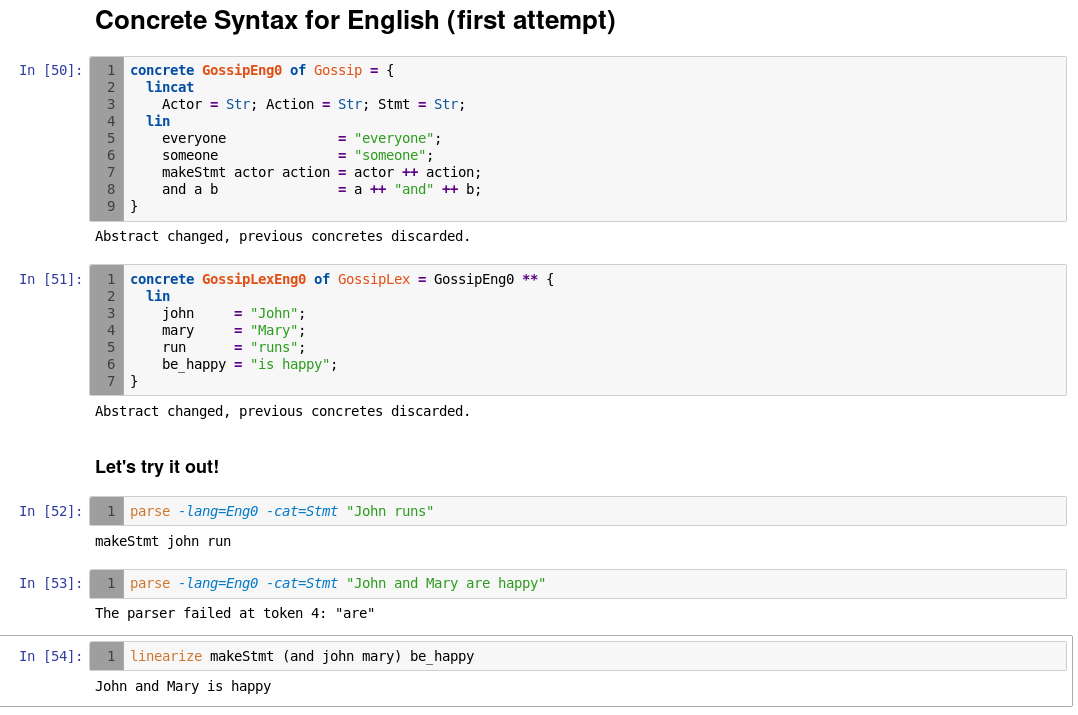
\includegraphics[scale=0.38]{screenshot_jupyter.png}
\end{frame}

\begin{frame}
    \frametitle{Describing the Fragment in \GF{} -- Concrete Syntax}

    \begin{block}{Problem}
        \str{John \textbf{is} happy} $\quad$ vs $\quad$ \str{John and Mary \textbf{are} happy}
    \end{block}

    \vspace{2em}
    \begin{block}{Solutions}
        \begin{itemize}
            \item More sophisticated grammar rules
            \item Use the \emph{resource grammar library}
        \end{itemize}
    \end{block}
\end{frame}

\begin{frame}[fragile]
    \frametitle{Describing the Fragment in \GF{} -- Concrete Syntax}

    \begin{lstlisting}[language=GF]
concrete GossipEng of Gossip = {
  param
    $\lcol{Plurality = Sg | Pl;}$
  lincat
    Actor  = {s : Str; $\lcol{p : Plurality}$};
    Action = $\lcol{Plurality}$ => Str;
    Stmt   = Str;
  lin
    everyone  = {s = "everyone"; $\lcol{p = Sg}$};
    someone   = {s = "someone"; $\lcol{p = Sg}$};
    makeStmt actor action = actor.s ++ action ! $\lcol{actor.p}$;
    twoOf a b = {s = a.s ++ "and" ++ b.s; $\lcol{p = Pl}$};
}
    \end{lstlisting}

    %\pause
    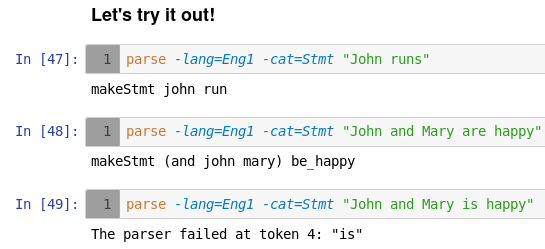
\includegraphics[scale=0.38]{screenshot_eng1.png}
\end{frame}

\begin{frame}[fragile]
    \frametitle{Describing the Fragment in \GF{} -- Concrete Syntax}
    \emph{Resource Grammar Library}: grammar rules for 36 languages

    \begin{lstlisting}[language=GF]
concrete GossipEng of Gossip = open SyntaxEng, DictEng in {
  lincat
    Actor  = NP;
    Action = VP;
    Stmt   = S;
  lin
    everyone  = everyone_NP;
    someone   = someone_NP;
    makeStmt actor action = mkS (mkCl actor action);
    twoOf a b = mkNP and_Conj a b;
}
    \end{lstlisting}
\end{frame}

\begin{frame}[fragile]
    \frametitle{Where are we?}
    % \frametitle{Describing the Fragment in \GF{}}
    \begin{minipage}{0.25\textwidth}\centering\str{John and Mary are happy}\end{minipage} $\;\mapsto\;$ 
    \resizebox{0.35\textwidth}{!}{
        \begin{tikzpicture}[baseline=0.0em]
            \node[line width=0,rounded corners=.2cm,fill=gray!25] (abs) at (0,0) {
                \begin{tikzpicture}
                    \node (a) at (-1, 0) {\gfinline{twoOf}};
                    \node (j) at (-1.6, -.8) {\gfinline{john}};
                    \node (m) at (-.4, -.8) {\gfinline{mary}};
                    \node (h) at (1, 0) {\gfinline{be_happy}};
                    \node (s) at (0, .8) {\gfinline{makeStmt}};
                    \draw (a) -- (s);
                    \draw (h) -- (s);
                    \draw (a) -- (j);
                    \draw (a) -- (m);
                \end{tikzpicture}
            };
        \end{tikzpicture}
    }

    %\pause
    \vspace{2em}
    \resizebox{\textwidth}{!}{
        \begin{tikzpicture}[xscale=1.3]
            \draw[white,line width=0,rounded corners=.2cm,fill=blue!25] (-5,3.5) rectangle (-0.1,-0.5);
            \draw[white,line width=0,rounded corners=.2cm,fill=green!25] (0.1,3.5) rectangle (5,-0.5);
            \node (gf) at (-2.5,--0.25) {\begin{tabular}{c}\textbf{\GF}\\(Grammatical Framework)\end{tabular}};
            \node (gf) at (2.5,--0.25) {\textbf{\MMT}};
            \node[draw,minimum width=2cm] (utt) at (-3.5,1.8) {NL Utterance};
            \draw[] (-1,1) -- (0,3) -- (1,1) -- cycle;
            \node[ellipse,line width=1mm,draw=red] (st) at (0,1.5) {\begin{tabular}{c}Syntax\\Tree\end{tabular}};
            \draw[->] (-2.5, 1.8) to[bend left=15] node[above] {parsing} (-0.8,1.8);
            \draw (2.5,1) -- (3.5,3) -- (4.5,1) -- cycle;
            \node (qlf) at (3.5,1.5) {\begin{tabular}{c}Logic\\Expression\end{tabular}};
            \draw[->] (0.8,1.8) to[bend left=15] node[above] {Semantics} node[below]{Construction} (2.7,1.8);
        \end{tikzpicture}
    }
\end{frame}

\begin{frame}
    \frametitle{\MMT{} -- ``anything you can do we can do meta''~\cite{RabKoh:WSMSML13}}
    \begin{itemize}
        \item You may remember ``Rapid Prototyping Formal Systems in MMT: 5 Case Studies''~\cite{MueRab:rpfsm}
        \item Meta meta theories/meta meta tool set
        \item Little theories
        \item Bring your own logic
        \item Logic development environment
        \item Foundation-independent
    \end{itemize}
\end{frame}

\begin{frame}[fragile]
    \frametitle{From \GF{} to \MMT{}}

    \begin{minipage}{0.49\textwidth}
        Abstract syntax (\GF)
        
        \vspace{0.6em}
        \lstinputlisting[language=GF]{snippets/Gossip.gf}
    \end{minipage}
    \begin{minipage}{0.47\textwidth}
        Language theory (\MMT)

        \vspace{0.6em}
        \lstinputlisting[language=MMT]{snippets/Gossip.mmt}
    \end{minipage}

    %\pause
    \vspace{0.4em}
    \resizebox{0.35\textwidth}{!}{
        \begin{tikzpicture}[baseline=0.0em]
            \node[line width=0,rounded corners=.2cm,fill=gray!25] (abs) at (0,0) {
                \begin{tikzpicture}
                    \node (a) at (-1, 0) {\gfinline{twoOf}};
                    \node (j) at (-1.6, -.8) {\gfinline{john}};
                    \node (m) at (-.4, -.8) {\gfinline{mary}};
                    \node (h) at (1, 0) {\gfinline{be_happy}};
                    \node (s) at (0, .8) {\gfinline{makeStmt}};
                    \draw (a) -- (s);
                    \draw (h) -- (s);
                    \draw (a) -- (j);
                    \draw (a) -- (m);
                \end{tikzpicture}
            };
        \end{tikzpicture}
    }
    $\;\;\mapsto\;\;$ \mmtstyle{makeStmt (twoOf john mary) be\_happy}
\end{frame}

\begin{frame}[fragile]
    \frametitle{Where are we?}

    \resizebox{0.7\textwidth}{!}{
        \begin{tikzpicture}[baseline=0.0em]
            \node[line width=0,rounded corners=.2cm,fill=blue!25] (abs) at (0,0.5) {\mmtstyle{makeStmt (twoOf john mary) be\_happy}};
            \node[line width=0,rounded corners=.2cm,fill=green!25] (term) at (0,-0.5) {\mmtstyle{makeStmt (twoOf john mary) be\_happy}};
            \node[align=center] (str) at (-5,0) {``\textit{John and Mary}\\\textit{are happy}''};

            \draw[->] (abs) -- (term);
            \draw[->] (str) -- (abs);
        \end{tikzpicture}
    }

    \vspace{2em}
    \resizebox{\textwidth}{!}{
        \begin{tikzpicture}[xscale=1.3]
            \draw[white,line width=0,rounded corners=.2cm,fill=blue!25] (-5,3.5) rectangle (-0.1,-0.5);
            \draw[white,line width=0,rounded corners=.2cm,fill=green!25] (0.1,3.5) rectangle (5,-0.5);
            \node (gf) at (-2.5,--0.25) {\begin{tabular}{c}\textbf{\GF}\\(Grammatical Framework)\end{tabular}};
            \node (gf) at (2.5,--0.25) {\textbf{\MMT}};
            \node[draw,minimum width=2cm] (utt) at (-3.5,1.8) {NL Utterance};
            \draw[] (-1,1) -- (0,3) -- (1,1) -- cycle;
            \node[] (st) at (0,1.5) {\begin{tabular}{c}Syntax\\Tree\end{tabular}};
            \draw[->] (-2.5, 1.8) to[bend left=15] node[above] {parsing} (-0.8,1.8);
            \draw (2.5,1) -- (3.5,3) -- (4.5,1) -- cycle;
            \node[ellipse,draw=red,line width=1mm] (qlf) at (3.5,1.5) {\begin{tabular}{c}Logic\\Expression\end{tabular}};
            \draw[->] (0.8,1.8) to[bend left=15] node[above] {Semantics} node[below]{Construction} (2.7,1.8);
        \end{tikzpicture}
    }

\end{frame}

\begin{frame}[fragile]
    \frametitle{Target Logic and Domain Theory in \MMT}
    \lstinputlisting[language=MMT]{snippets/FOL_Syntax.mmt}
    %\pause
    \lstinputlisting[language=MMT]{snippets/DomainTheory.mmt}
\end{frame}

\begin{frame}[fragile]
    \frametitle{Where are we?}

    \resizebox{\textwidth}{!}{
        \begin{tikzpicture}[baseline=0.0em]
            \node[line width=0,rounded corners=.2cm,fill=blue!25] (abs) at (0,0.5) {\mmtstyle{makeStmt (twoOf john mary) be\_happy}};
            \node[line width=0,rounded corners=.2cm,fill=green!25] (term) at (0,-0.5) {\mmtstyle{makeStmt (twoOf john mary) be\_happy}};
            \node[align=center] (str) at (-5,0) {``\textit{John and Mary}\\\textit{are happy}''};
            \node (log) at (6, 0) {\mmtstyle{(happy' john')$\land$(happy' mary')}};
            \draw[->] (abs) -- (term);
            \draw[->] (str) -- (abs);
            \draw[dashed,->,ultra thick,red] (term) -- (log);
        \end{tikzpicture}
    }

    \vspace{2em}
    \resizebox{\textwidth}{!}{
        \begin{tikzpicture}[xscale=1.3]
            \draw[white,line width=0,rounded corners=.2cm,fill=blue!25] (-5,3.5) rectangle (-0.1,-0.5);
            \draw[white,line width=0,rounded corners=.2cm,fill=green!25] (0.1,3.5) rectangle (5,-0.5);
            \node (gf) at (-2.5,--0.25) {\begin{tabular}{c}\textbf{\GF}\\(Grammatical Framework)\end{tabular}};
            \node (gf) at (2.5,--0.25) {\textbf{\MMT}};
            \node[draw,minimum width=2cm] (utt) at (-3.5,1.8) {NL Utterance};
            \draw[] (-1,1) -- (0,3) -- (1,1) -- cycle;
            \node[] (st) at (0,1.5) {\begin{tabular}{c}Syntax\\Tree\end{tabular}};
            \draw[->] (-2.5, 1.8) to[bend left=15] node[above] {parsing} (-0.8,1.8);
            \draw (2.5,1) -- (3.5,3) -- (4.5,1) -- cycle;
            \node (qlf) at (3.5,1.5) {\begin{tabular}{c}Logic\\Expression\end{tabular}};
            \draw[->] (0.8,1.8) to[bend left=15] node[above] {Semantics} node[below]{Construction} (2.7,1.8);
            \node[ellipse,draw=red,line width=1mm,minimum width=2.5cm,minimum height=1.8cm] at (1.75,1.9) {};
        \end{tikzpicture}
    }

\end{frame}

\begin{frame}
    \frametitle{Semantics Construction in \MMT}
    \begin{tikzpicture}
        \node[thy] (gossip) at (0, 0) {$\mmtthy{\textbf{Gossip}}{Actor, Action, Stmt}{everyone, someone,\\makeStmt, twoOf}$};
        \node[thy] (gossipLex) at (0, -3) {$\mmtthy{\textbf{GossipLex}}{}{john, mary,\\run, be\_happy}$};
        \node[thy] (fol) at (6, 0) {$\mmtthy{\textbf{FOL}}{o, \iota}{\land, \neg, \lor\\\forall, \exists}$};
        \node[thy] (dt) at (6, -3) {$\mmtthy{\textbf{DomainTheory}}{}{john', mary',\\run', happy'}$};

        \draw[include] (gossip) -- (gossipLex);
        \draw[meta] (fol) -- (dt);
        %\only<2->{\draw[view] (gossipLex) -- (dt);}
        %\only<3>{\draw[view] (gossip) -- (dt);}
        %\only<4>{\draw[view] (gossip) -- (fol);}
        {\draw[view] (gossipLex) -- (dt);}
        {\draw[view] (gossip) -- (fol);}
    \end{tikzpicture}
\end{frame}

\begin{frame}[fragile]
    \frametitle{Naive Approach}

    \lstinputlisting[language=MMT]{snippets/GossipSem0.mmt}
\end{frame}

\begin{frame}[fragile]
    \frametitle{Type Raising~\cite{Montague:tptoqi73}}
    
    \begin{block}{Problem}
        \mmtstyle{Actor = $\iota$}

        \mmtstyle{everyone : Actor = ?} 
    \end{block}

    \vspace{1em}
    \begin{block}{Solution}
        \mmtstyle{Actor = ($\iota$ \jraa{} o) \jraa{} o}

        \mmtstyle{john = [$\varphi$] $\varphi$ john'}

        \mmtstyle{everyone = [$\varphi$] $\forall$ [x] ($\varphi$ x) = [$\varphi$] $\forall$ $\varphi$}
    \end{block}

    \vspace{1em}
    \begin{block}{Example}
        \str{everyone runs}
        $\;\,\mapsto\;\,$ \mmtstyle{([$\varphi$] $\forall$ [x] ($\varphi$ x)) run'}
        $\;\;\leadsto_\beta\;\;$ \mmtstyle{$\forall$ [x] (run' x)}
    \end{block}
\end{frame}

\begin{frame}[fragile]
    \frametitle{Better Approach}

    \lstinputlisting[language=MMT]{snippets/GossipSem.mmt}


    \only<2>{
    \textblockcolor{white}
    \begin{textblock*}{120mm}(9mm,57mm)
        These views are described in NL semantics papers like~\cite{Montague:tptoqi73}:

        \vspace{0.5em}
        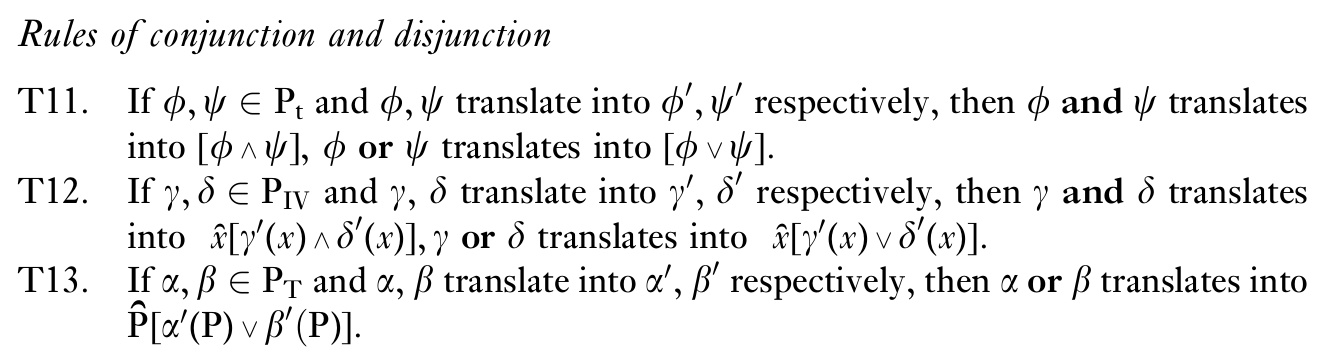
\includegraphics[scale=0.2]{montague.png}
    \end{textblock*}
    \textblockcolor{}
    }
\end{frame} 

\def\myarr#1{\vspace{0.4em}$\quad\quad\quad\quad\downarrow$ \footnotesize{#1}\vspace{0.4em}}
\begin{frame}
    \frametitle{Example}
    \str{John and Mary are happy}

    \vspace{0.4em}$\;\,\quad\quad\quad\downarrow$ \footnotesize{parse}\vspace{0.4em}

    \mmtstyle{makeStmt (twoOf john mary) be\_happy}

    \myarr{semantics construction}

    \mmtstyle{([a,$\varphi$] a $\varphi$)}

    \vspace{-0.3em}
    \mmtstyle{$\quad$(([a1,a2] [$\varphi$] (a1 $\varphi$) $\land$ (a2 $\varphi$)) ([$\varphi$] $\varphi$ john') ([$\varphi$] $\varphi$ mary'))}

    \vspace{-0.3em}
    \mmtstyle{$\quad$([x] happy' x)}

    \myarr{simplify}

    \mmtstyle{([a1,a2,$\varphi$] (a1 $\varphi$) $\land$ (a2 $\varphi$)) ([$\varphi$] $\varphi$ john') ([$\varphi$] $\varphi$ mary') happy'}

    \myarr{simplify}

    \mmtstyle{([$\varphi$] ($\varphi$ john') $\land$ ($\varphi$ mary')) happy'}

    \myarr{simplify}

    \mmtstyle{(happy' john') $\land$ (happy' mary')}
\end{frame}

\begin{frame}
    \frametitle{Other Examples (from paper)}
    \begin{block}{Adding Transitive Verbs ($\leadsto$ more type raising)}
        \str{John and Mary love everyone}

        \myarr{}

        \mmtstyle{$\forall$[x:$\iota$](love' john' x)$\land$(love' mary' x)}
    \end{block}
\end{frame}

\begin{frame}
    \frametitle{Other Examples (from paper)}
    \vspace{2em}
    \begin{block}{(Multi) Modal Logic}
        Modalities:
        \begin{itemize}
            \item \emph{deontic} -- something is obligatory (\mmtstyle{$\llbracket$d$\rrbracket$}) or permissible (\mmtstyle{$\llangle$d$\rrangle$})
            \item \emph{epistemic} -- someone believes something is true (\mmtstyle{$\llbracket$e john'$\rrbracket$}) or possible (\mmtstyle{$\llangle$e john'$\rrangle$}).
        \end{itemize}
        \vspace{1.5em}
        \str{John doesn't believe that Mary has to run}

        \myarr{}

        \mmtstyle{$\neg$$\llbracket$(e john')$\rrbracket$$\llbracket$d$\rrbracket$(run' mary')}.
    \end{block}
\end{frame}

\begin{frame}[fragile]
    \frametitle{\GLF{} Script}

    \lstinputlisting[language=MMT]{snippets/glf_log.txt}
\end{frame}

\begin{frame}
    \frametitle{Conclusions}
    \begin{itemize}
        \item \GLF = tool to implement NLU system
        \item would have been great in the 90's to avoid pen-and-paperness
        \item previous versions used for teaching NL semantics
    \end{itemize}

    \vspace{2em}
    \begin{itemize}
        \item work on a Jupyter kernel for GLF
        \item generic tableau calculus for semantic analysis?
    \end{itemize}
\end{frame}

\begin{frame}[fragile]
    \frametitle{The Grammatical Logical Framework (\GLF)}
\resizebox{\textwidth}{!}{
    \begin{tikzpicture}[xscale=1.3]
        \draw[white,line width=0,rounded corners=.2cm,fill=blue!25] (-5,3.5) rectangle (-0.1,-0.5);
        \draw[white,line width=0,rounded corners=.2cm,fill=green!25] (0.1,3.5) rectangle (5,-0.5);
        \node (gf) at (-2.5,--0.25) {\begin{tabular}{c}\textbf{\GF}\\(Grammatical Framework)\end{tabular}};
        \node (gf) at (2.5,--0.25) {\textbf{\MMT}};

        \node[draw,minimum width=2cm] (utt) at (-3.5,1.8) {NL Utterance};
        \draw[] (-1,1) -- (0,3) -- (1,1) -- cycle;
        \node[] (st) at (0,1.5) {\begin{tabular}{c}Syntax\\Tree\end{tabular}};
        \draw[->] (-2.5, 1.8) to[bend left=15] node[above] {parsing} (-0.8,1.8);
        \draw (2.5,1) -- (3.5,3) -- (4.5,1) -- cycle;
        \node (qlf) at (3.5,1.5) {\begin{tabular}{c}Logic\\Expression\end{tabular}};
        \draw[->] (0.8,1.8) to[bend left=15] node[above] {Semantics} node[below]{Construction} (2.7,1.8);
        \node (lf) at (2.0, -1.5) {\begin{tabular}{c}Transition trivial:\\compatible logical frameworks\end{tabular}};
        \draw[->] (lf) to[bend left=15] (0.0, 0.9);
    \end{tikzpicture}
    }

    \vspace{2em}
    \begin{columns}
        \begin{column}{0.71\textwidth}
            \resizebox{\textwidth}{!}{
                \begin{tabular}{r@{\hskip3pt} l l}
                    \vspace{0.1em}&\textbf{\GF} &\textit{= \textbf{grammar} development framework}\\
                    \vspace{0.1em}+&\textbf{\MMT} &\textit{= \textbf{logic} development framework}\\
                    \hline
                    \\[-1em]
                    &\textbf{\GLF} &\textit{= \textbf{semantics} development framework}\\
                \end{tabular}
            }
        \end{column}
        \begin{column}{0.28\textwidth}
            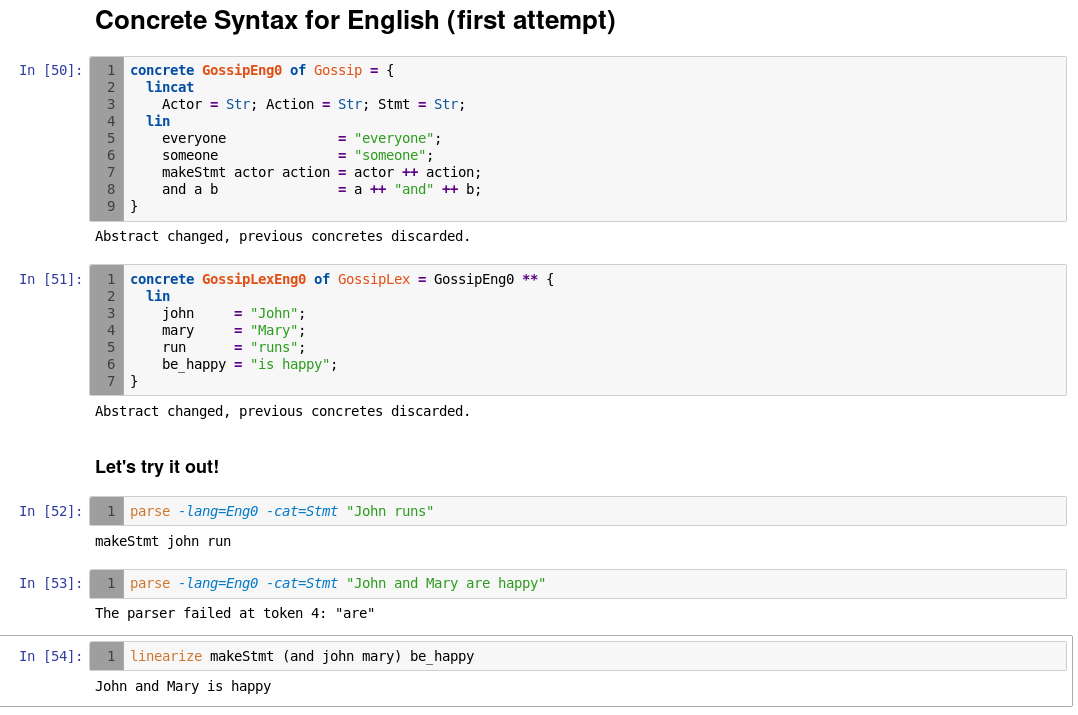
\includegraphics[scale=0.09]{screenshot_jupyter.png}
        \end{column}
    \end{columns}

\end{frame}

\begin{frame}
    \frametitle{Bonus: Compositionality}
    
    Problem:

    \str{John owns a book. It is red.}

    \log{$(\exists x.\text{own'}(\text{john'}, x) \land \text{book'}(x)) \land \text{red}(x)$}

    \vspace{1em}
    Solution: Define more suitable logic (e.g. discourse representation theory)
\end{frame}

\begin{frame}
    \frametitle{Bonus: Lexical Ambiguity}
    
    \str{Mary works at a bank}

    \vspace{1em}
    $\leadsto$ river bank or bank institute?

    \vspace{1em}
    $\leadsto$ two parse trees:
    \begin{itemize}
        \item \gfinline{work_at mary bank_institute}
        \item \gfinline{work_at mary bank_river}
    \end{itemize}
\end{frame}

\begin{frame}
    \frametitle{Bonus: Structural Ambiguity}
    
    \str{Mary saw the man with the binoculars}

    \vspace{1em}
    \begin{minipage}[t]{0.5\textwidth}
        \scalebox{0.6}{
            \Tree [ .S [ .NP \textit{Mary} ] [ .VP \textit{saw} [ .NP \textit{the} [ .CN \textit{man} [ .Adv \edge[roof]; \textit{with the binoculars} ] ] ] ] ]
        }
    \end{minipage}\hfill
    \begin{minipage}[t]{0.5\textwidth}
        \scalebox{0.6}{
            \Tree [ .S [ .NP \textit{Mary} ] [ .VP [ .VP \textit{saw} [ .NP \textit{the} [ .CN \textit{man} ] ] ] [ .Adv \edge[roof]; \textit{with the binoculars} ] ] ]
        }
    \end{minipage}
\end{frame}

\begin{frame}[allowframebreaks]
    \frametitle{References}
    \bibliography{kwarc}
\end{frame}

\end{document}
